%%%%%%%%%%%%%%%%%%%%%%%%%%%%%%%%%%%%%%%%%
% University Assignment Title Page 
% LaTeX Template
% Version 1.0 (27/12/12)
%
% This template has been downloaded from:
% http://www.LaTeXTemplates.com
%
% Original author:
% WikiBooks (http://en.wikibooks.org/wiki/LaTeX/Title_Creation)
%
% License:
% CC BY-NC-SA 3.0 (http://creativecommons.org/licenses/by-nc-sa/3.0/)
% 
% Instructions for using this template:
% This title page is capable of being compiled as is. This is not useful for 
% including it in another document. To do this, you have two options: 
%
% 1) Copy/paste everything between \begin{document} and \end{document} 
% starting at \begin{titlepage} and paste this into another LaTeX file where you 
% want your title page.
% OR
% 2) Remove everything outside the \begin{titlepage} and \end{titlepage} and 
% move this file to the same directory as the LaTeX file you wish to add it to. 
% Then add \input{./title_page_1.tex} to your LaTeX file where you want your
% title page.
%
%%%%%%%%%%%%%%%%%%%%%%%%%%%%%%%%%%%%%%%%%

%----------------------------------------------------------------------------------------
%	PACKAGES AND OTHER DOCUMENT CONFIGURATIONS
%----------------------------------------------------------------------------------------

\documentclass[12pt]{article}
\usepackage{graphicx}
\usepackage{caption}
\usepackage{subcaption}
\begin{document}
\begin{titlepage}

\newcommand{\HRule}{\rule{\linewidth}{0.5mm}} % Defines a new command for the horizontal lines, change thickness here

\center % Center everything on the page
 
%----------------------------------------------------------------------------------------
%	HEADING SECTIONS
%----------------------------------------------------------------------------------------

\textsc{\LARGE McGill University}\\[1.5cm] % Name of your university/college
\textsc{\Large COMP 521}\\[0.5cm] % Major heading such as course name
\textsc{\large Modern Computer Games}\\[0.5cm] % Minor heading such as course title

%----------------------------------------------------------------------------------------
%	TITLE SECTION
%----------------------------------------------------------------------------------------

\HRule \\[0.4cm]
{ \huge \bfseries TerraGen: Procedural Terrain Generation and Resource Analysis}\\[0.4cm] % Title of your document
\HRule \\[1.0cm]
 
%----------------------------------------------------------------------------------------
%	AUTHOR SECTION
%----------------------------------------------------------------------------------------

\begin{minipage}{0.4\textwidth}
\begin{flushleft} \large
Benjamin \textsc{San Souci} \\ % Your name
Maude \textsc{Lemaire} % Your name
\end{flushleft}
\end{minipage}
~
\begin{minipage}{0.4\textwidth}
\end{minipage}\\[4cm]

% If you don't want a supervisor, uncomment the two lines below and remove the section above
%\Large \emph{Author:}\\
%John \textsc{Smith}\\[3cm] % Your name

%----------------------------------------------------------------------------------------
%	DATE SECTION
%----------------------------------------------------------------------------------------

{\large \today}\\[3cm] % Date, change the \today to a set date if you want to be precise

%----------------------------------------------------------------------------------------
%	LOGO SECTION
%----------------------------------------------------------------------------------------

%\includegraphics{Logo}\\[1cm] % Include a department/university logo - this will require the graphicx package
 
%----------------------------------------------------------------------------------------

\vfill % Fill the rest of the page with whitespace

\end{titlepage}

\section{Introduction}

TerraGen aims to generate realistic island terrains using a relaxed polygonal map and assigning biomes based on simulated moisture and elevation. Following the map generation process, the city generation algorithm analyzes the terrain and produces a  set of cities with unique statistics directly related to their location and access to resources. 

Island generation was modeled after Amit Patel's ``Polygonal Map Generation for Games''\cite{Patel:2010:Online}, where Chrisophe Le Besnerais's JavaScript version, ``Island.js''\cite{LeBesnec:2015:Online} was extended to accommodate for additional features. First a graph structure of polygons is generated, then annotated with elevation, moisture, and labeled as either land or water. In order to generate a more natural-looking island, Voronoi polygons were generated and relaxed using an implementation by Raymond Hill \cite{Hill:2015:Online}. Extensions to the implementation included adding fishing regions, minerals, volcanoes, tectonic plates, forest density, and fauna abundance. 

The TerraGen city statistic generation addresses a problem that has been little discussed in the scope of games beyond the intersection of geography information systems (GIS) and 3D game engines. Using the generated plot, the city generation algorithm finds a suitable location at which to place a city. From this location, resources in close proximity are identified and used in determining the city's population size, army size, happiness level and wealth, among other features. 

The result is a randomly generated island with over two dozen biomes, oceanic regions, dispered minerals and a handful of cities. A sample map at different stages of generation is included in the methodology portion of the report. 

The project was separated into two major components: the terrain generation and extensions, and the city statistics generation. Maude was mainly responsible for the terrain generation portion of the project and the majority of the final report. Benjamin produced the city generation algorithm. 

\section{Background}
Map generation has been a important focus within the gaming industry in recent years as a means of promoting re-playability without having to manually generate a large number of maps. By randomly generating a map with new instances of a game, the players must face new challenges and adapt their game-play to suit the new terrain. A wide range of approaches already exist, with varying levels of complexity and randomness.

\subsection{Grids}
Terrains are typically built off of a grid system; this can be a simple tile-based square grid, a hexagonal grid, or a polygonal grid either composed of randomly sized convex shapes or relaxed polygons. Figure 1 displays the difference between each of these grid types and how ``natural'' each of these appear in island generation.

\begin{figure}
        \centering
        \begin{subfigure}[b]{0.45\textwidth}
                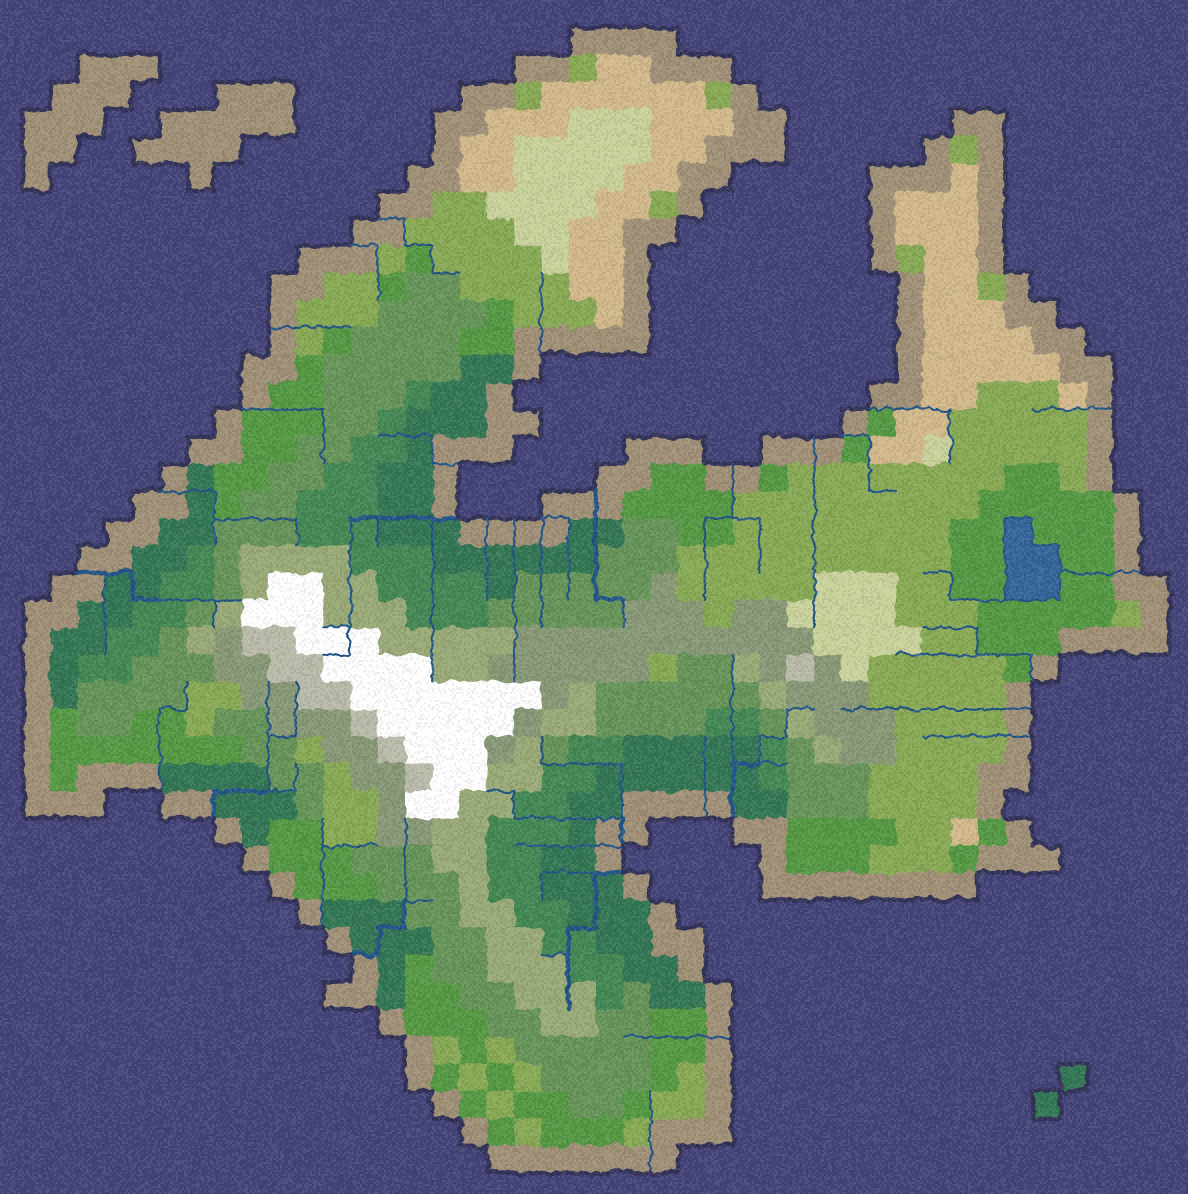
\includegraphics[width=\textwidth]{Square.png}
                \caption{Square Grid}
                \label{fig:Square}
        \end{subfigure}%
        ~ %add desired spacing between images, e. g. ~, \quad, \qquad, \hfill etc.
          %(or a blank line to force the subfigure onto a new line)
        \begin{subfigure}[b]{0.45\textwidth}
                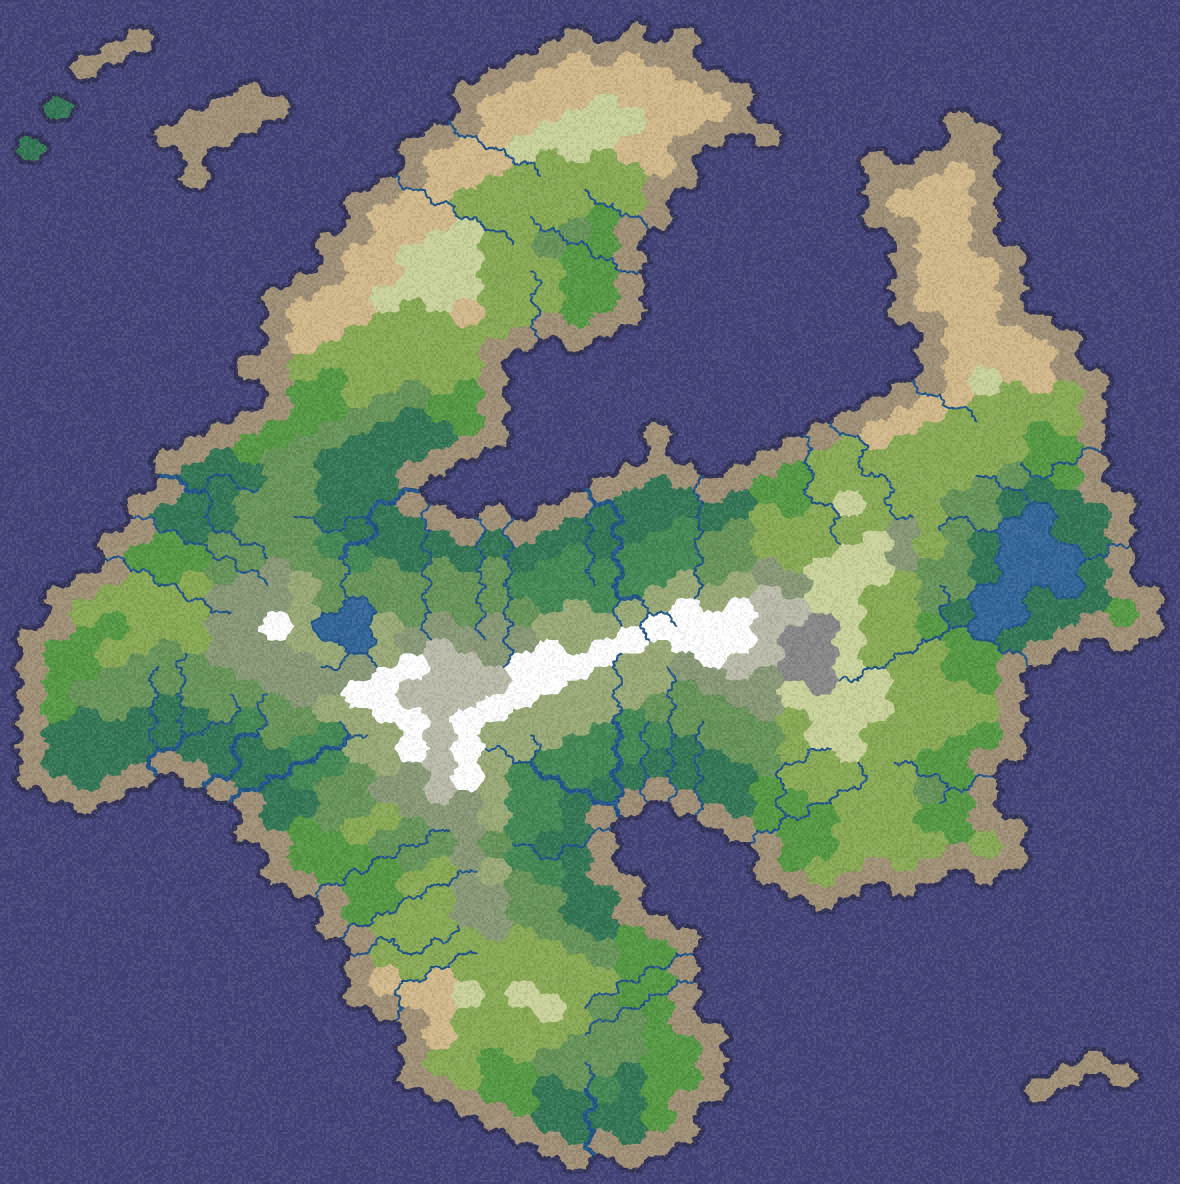
\includegraphics[width=\textwidth]{Hex.png}
                \caption{Hexagonal Grid}
                \label{fig:Hex}
        \end{subfigure}
        ~ %add desired spacing between images, e. g. ~, \quad, \qquad, \hfill etc.
          %(or a blank line to force the subfigure onto a new line)
        \begin{subfigure}[b]{0.45\textwidth}
                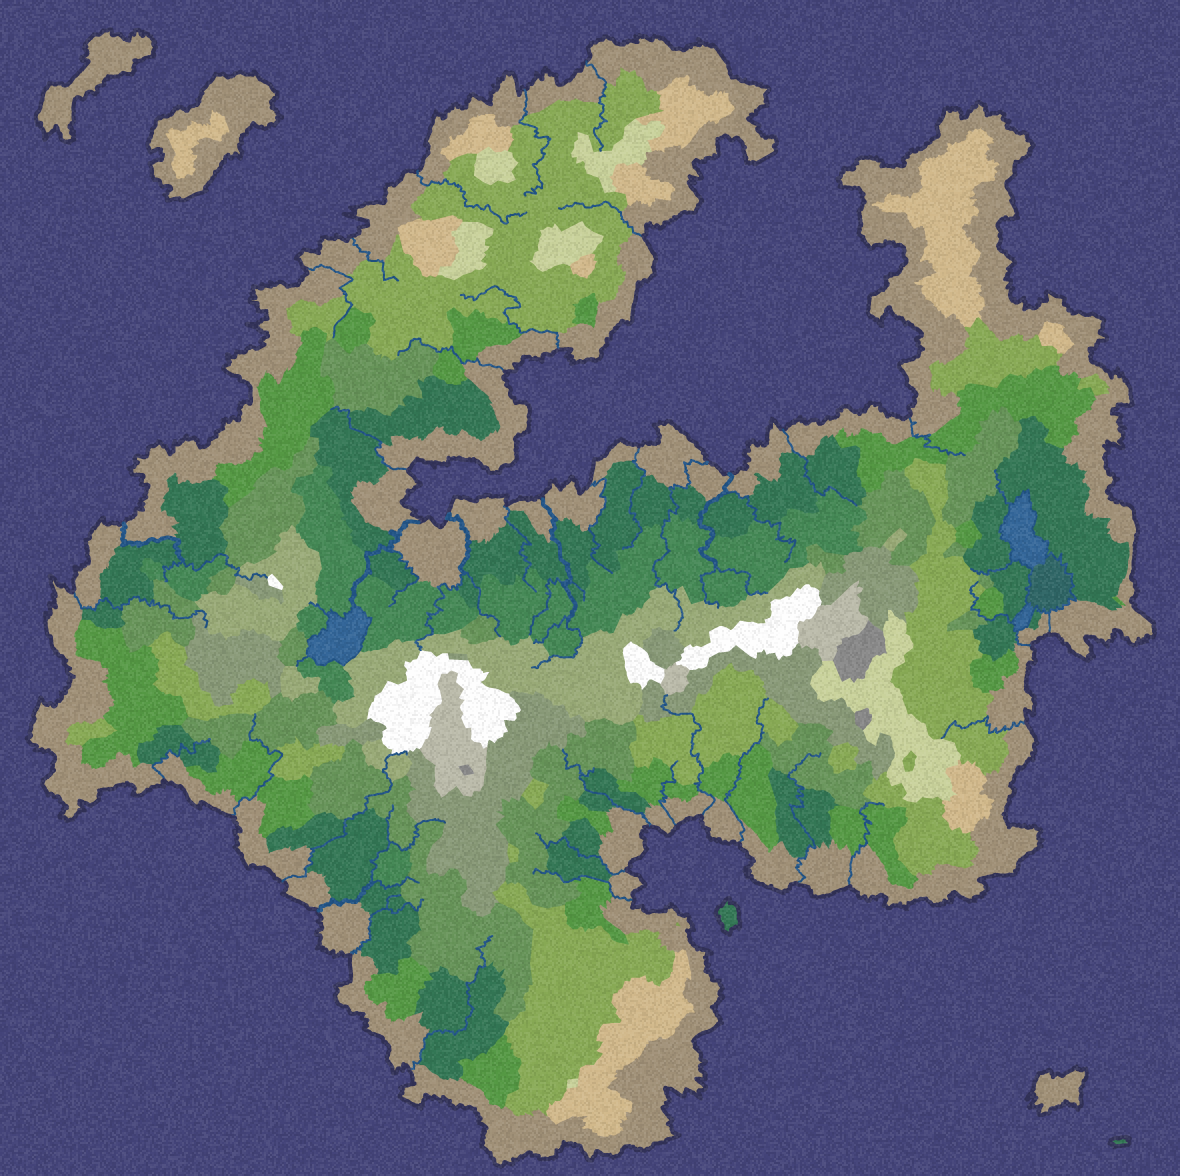
\includegraphics[width=\textwidth]{Random.png}
                \caption{Random Polygon Grid}
                \label{fig:Random}
        \end{subfigure}
        \begin{subfigure}[b]{0.45\textwidth}
                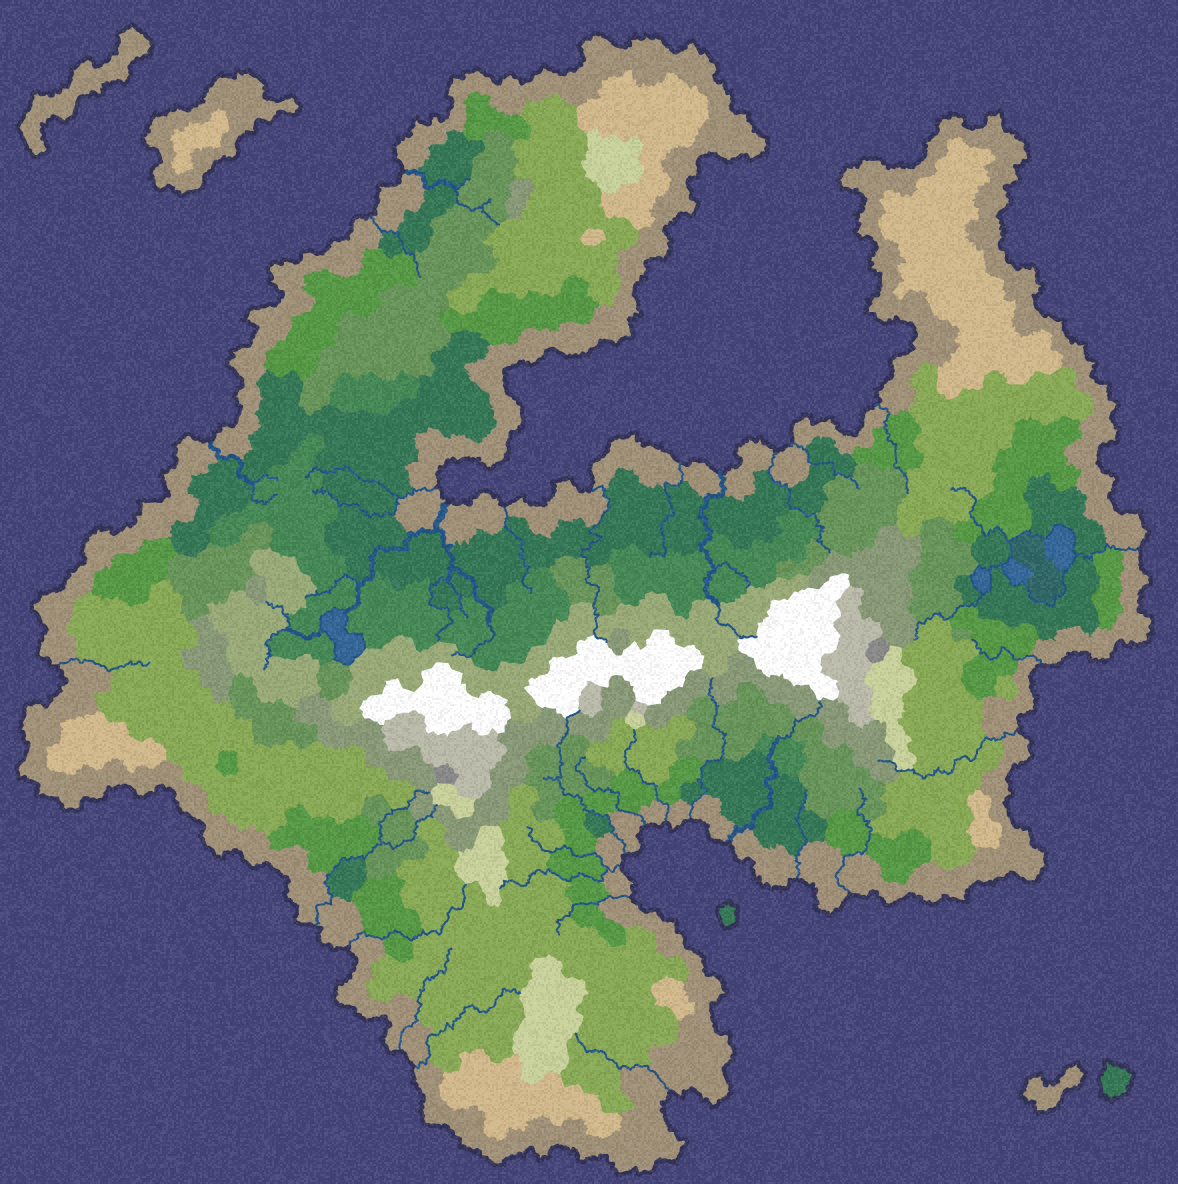
\includegraphics[width=\textwidth]{Relaxed.png}
                \caption{Relaxed Polygon Grid}
                \label{fig:Relaxed}
        \end{subfigure}
        \caption{Islands generated using Amit Patel's demo. Each is generated using Perlin noise, displays biomes, and demonstrates the use of different grid types.}\label{fig:gridtypes}
\end{figure}

Hexagonal grids and polygonal grids typically provide the most natural-looking islands. Hexagonal grids have been extensively developed by academics such as Clark Verbrugge\cite{Verbrugge:1997:Online}, and can be perturbed to add irregularity. Polygonal grid generation has mainly revolved around randomly generating a series of Voronoi polygons. A number of algorithms generate Voronoi diagrams based on a set of random points (Fortune's algorithm\cite{Fortune:1986:SAV:10515.10549}), a set area (Lloyd's algorithm\cite{doi:10.1137/S0036144599352836}) or Delaunay triangulations (Bowyer-Watson algorithm\cite{Watson01011981}). In particular, the set of points upon which the polygons are generated can be mapped to known natural phenomena. For example, researchers at the Universit\'{e} de Lyon,generated Voronoi diagrams based on hydrology \cite{Genevaux:2013:TGU:2461912.2461996}. As an extension, Lloyd relaxation can be used to distribute points more evenly for diagram generation. 

Following Patel's polygonal map generation methods, once a Voronoi diagram is generated, the internal representation consists of nodes and edges; the first is used for identifying adjacent polygons. The second represents the Delaunay triangulation which can be used for pathfinding. Conceptually, every corner in the triangulation corresponds to a polygon center and every edge to an edge in the diagram. As polygons in the map are irregular, it is difficult to make assumptions about neighboring cells and paths from one point to another; this representation ensures that the map is traversed in a meaningful way throughout the generation process. 

\subsection{Islands}

Realistic islands must maintain a rather circular shape, with some random variation. A radial function is suggested, using sine waves to produce a round island. The island is generated according to polar coordinates stemming from the center of the canvas. Depending on the sine waves, the island can resemble an octopus, with thin strips of land extended from the center of the island.  

Alternatively, Perlin noise can be generated and used to control the shape of the island given some constraints. This method provides more realistic island shapes due to the fact that Perlin noise consists of visual details of equal size; this gives a more controlled random appearance, closely imitating natural textures. 

Once land polygons have been identified, ocean is filled in from the edges and any remaining ``water'' polygons unreachable from the fringe of the map (landlocked) are marked as lakes. 

\subsubsection{Elevation}
In generating terrains, in order to provide a more realistic map, a natural-looking elevation must be assigned to each grid unit. Some typical approaches include using Perlin noise, real-world data, or fractal landscapes. 

\section{Methodology}

\section{Results}

\section{Conclusions \& Future Improvements}

\bibliographystyle{plain}
\bibliography{report.bib}
\end{document}